\documentclass[12pt,a4paper]{article}

% Essential packages
\usepackage[utf8]{inputenc}
\usepackage[T1]{fontenc}
\usepackage{amsmath,amsfonts,amssymb}
\usepackage{graphicx}
\usepackage{float}
\usepackage{cite}
\usepackage{url}
\usepackage{hyperref}
\usepackage{geometry}
\usepackage{setspace}
\usepackage{titlesec}
\usepackage{caption}
\usepackage{subcaption}
\usepackage{booktabs}
\usepackage{siunitx}
\usepackage{lineno}

% Page setup
\geometry{
    a4paper,
    margin=2.5cm,
    top=3cm,
    bottom=3cm
}

% Line spacing
\doublespacing

% Line numbers (uncomment if required by journal)
% \linenumbers

% Section formatting
\titleformat{\section}{\large\bfseries}{\thesection.}{1em}{}
\titleformat{\subsection}{\normalsize\bfseries}{\thesubsection.}{1em}{}

% Figure and table captions
\captionsetup{font=small,labelfont=bf}

% Hyperlink setup
\hypersetup{
    colorlinks=true,
    linkcolor=black,
    citecolor=blue,
    urlcolor=blue
}

% Title page information
\title{\textbf{The impact of forest management on the temperature sensitivity of SOC decomposition in a forest gradient from mediterranean to boreal}}

\author{
    First Author\textsuperscript{1,2}*, 
    Second Author\textsuperscript{1}, 
    Third Author\textsuperscript{3}\\
    \\
    \textsuperscript{1}Department of [Department], [University Name], [City, Country]\\
    \textsuperscript{2}[Second Affiliation if applicable]\\
    \textsuperscript{3}[Third Institution]\\
    \\
    *Corresponding author: email@institution.edu
}

\date{}

\begin{document}

\maketitle

\begin{abstract}
\noindent
\textbf{Background:} Provide context and rationale for your study. Briefly explain the problem or gap in knowledge that your research addresses.

\textbf{Methods:} Summarize your experimental design, key methods, and analytical approaches used in the study.

\textbf{Results:} Present the main findings of your research, including key quantitative results and statistical significance where applicable.

\textbf{Conclusions:} State the main conclusions and their broader implications. Highlight the significance of your findings and potential applications.

\textbf{Keywords:} keyword1, keyword2, keyword3, keyword4, keyword5
\end{abstract}

\newpage

\section{Introduction}


\subsection{Background and Rationale}


\subsection{Objectives and Hypotheses}

Clearly state your research objectives and hypotheses. For example:
\begin{itemize}
    \item \textbf{Primary objective:} To investigate the relationship between X and Y
    \item \textbf{Secondary objectives:} To evaluate Z and assess W
    \item \textbf{Hypothesis:} We hypothesize that X will significantly affect Y under conditions Z
\end{itemize}






\section{Materials and Methods}

\subsection{Holisoils study design}




\subsection{The database}



\subsection{Modeling SOC decomposition dependency on climate}

Provide detailed protocols that would allow others to reproduce your work. Use subsections for different experimental approaches:


\subsection{The model}

\subsubsection{The Bayesian framework}

\subsection{Implementation and hardware}




\section{Results}

% Example figure
\begin{figure}[H]
    \centering
    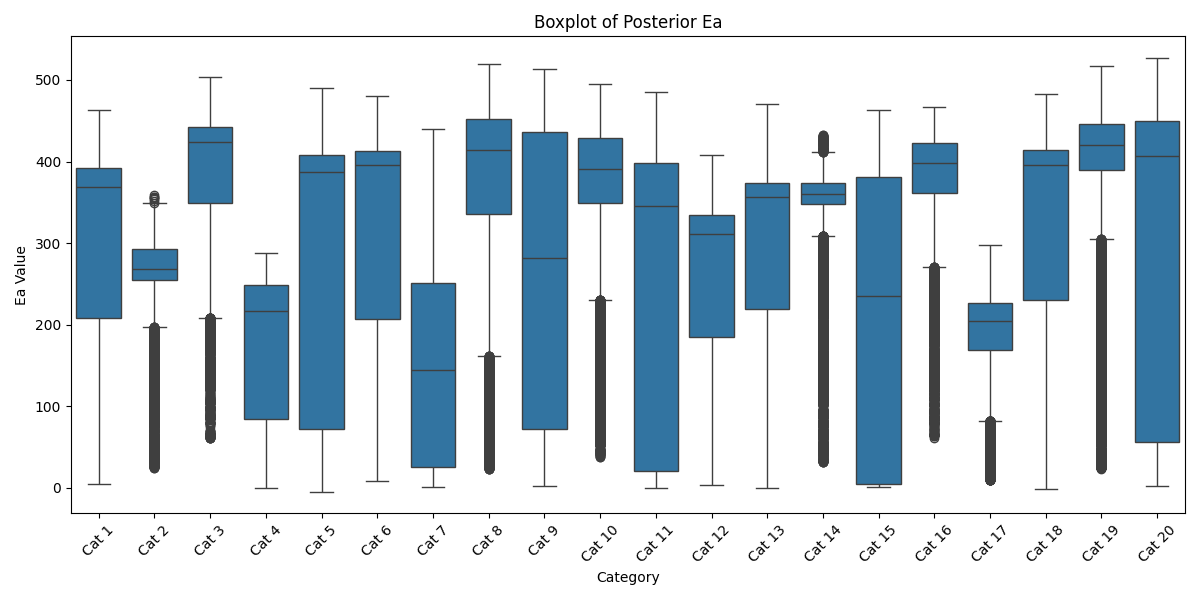
\includegraphics[width=0.8\textwidth]{"../E_0.png"}
    \caption{Example figure caption. Describe what the figure shows, including experimental conditions, sample sizes, and statistical tests. Error bars represent standard error of the mean. *p < 0.05, **p < 0.01.}
    \label{fig:example}
\end{figure}



\section{Discussion}

\subsection{Interpretation of Results}


\subsection{Limitations}

\subsection{Implications and Future Directions}



\section{Conclusions}

Summarize the key findings and their significance. Avoid simply repeating the abstract; instead, provide a synthesis that emphasizes the contribution of your work to the field.


\section*{Acknowledgments}

Acknowledge funding sources, institutional support, and individuals who contributed to the work but are not listed as authors.


\section*{Funding}

This work was supported by [Grant Agency] under Grant [Number]. [Author Name] was supported by [Fellowship/Scholarship].


\section*{Conflicts of Interest}

The authors declare no conflicts of interest.


\section*{Data Availability Statement}

The data that support the findings of this study are available from the corresponding author upon reasonable request [or specify repository/database where data are deposited].



% Bibliography
\bibliographystyle{plain}
\bibliography{references}


\end{thebibliography}

\end{document}